\documentclass[conference]{ieeetran}

%\IEEEoverridecommandlockouts
% The preceding line is only needed to identify funding in the first footnote. If that is unneeded, please comment it out.
\usepackage[section]{placeins}  % loads \FloatBarrier
\usepackage{cite}
\usepackage{amsmath,amssymb,amsfonts}
\usepackage{algorithmic}
\usepackage{graphicx}
\usepackage{textcomp}
\usepackage{xcolor}
\usepackage{booktabs, array}
\def\BibTeX{{\rm B\kern-.05em{\sc i\kern-.025em b}\kern-.08em
    T\kern-.1667em\lower.7ex\hbox{E}\kern-.125emX}}
    
%used for creating sub-figures    
\usepackage{subcaption}    

%http://www.texfaq.org/FAQ-balance
\usepackage{flushend}

% for external hyperlinks
\usepackage[colorlinks=true, urlcolor=blue]{hyperref}

%https://tex.stackexchange.com/questions/23313/how-can-i-reduce-padding-after-figure
\setlength{\belowcaptionskip}{-5pt}


\begin{document}

\title{Ghost Forest Capstone Final Paper}



%Begin enumeration of author names with a unique mark for each affliation
%Note: There must be no spaces between the end of the Name IEEEAuthorN block and Affliataion IEEEAuthorBlockA block
\author{\IEEEauthorblockN{
Mahin Ganesan,
Brendan Jalali,
Tom Lever,
and Nicholas Miller}\IEEEauthorblockA{
School of Data Science\\
University of Virginia, Charlottesville, VA\\
Repositories: \href{https://github.com/tslever/Ghost\_Forest\_Detection}{Ghost Forest Detection}, 
\href{https://github.com/tslever/urban-tree-detection}{urban-tree-detection}, 
\href{https://github.com/tslever/urban-tree-detection-data}{urban-tree-detection-data}
}}

\maketitle


\section{Abstract}

This project aims to identify ghost forests across the East Coast of the United States using deep learning algorithms for image detection. Ghost forests are areas with more than 10 dead trees per hectare, and their locations are currently largely unknown. To predict dead trees, we have adapted an existing urban tree detection neural network \cite{ventura2024individual} to predict the centroids of dead trees in satellite images, achieving an F1 score of 0.795. Overall, the goal of this project is for the members to participate in developing a data science pipeline to identify ghost forests, which will provide us with an understanding of where and why ghost forest hot spots may arise. By knowing where ghost forests occur, governments and localities can push for legislation to keep these forests from dying, allowing them to continue protecting the surrounding coastal communities and ecosystems. 
 
\section{Introduction}

For the study and preservation of coastal forests \cite{ventura2024individual}, our sponsors, researchers in the Department of Environmental Science at the University of Virginia, have taken an interest in developing a tool that will be able to identify ghost forests across the country. Our model, which predicts the locations of dead trees in ghost forests, is a key step in understanding the mechanisms behind forest decline due to saltwater intrusion. The results of this improved model will lead to a better understanding of the systems that cause the death of these forests. The primary research questions that we answered with this project include: 
\begin{enumerate}
    \item How can we best identify ghost forests in the United States?
    \item How do we build a data pipeline to process satellite imagery for our model?
    \item How do we optimize our model to identify dead trees?
\end{enumerate}

\section{Background/Related Work}

Ghost forest tree prediction is a novel concept with limited prior research. To address this, we instead adapted techniques from the broader field of individual tree detection in remote sensing imagery to guide our methods.

The primary foundation of our approach is the urban tree detection model developed by Ventura et al. that used a CNN approach for large-scale tree detection using multispectral imagery\cite{ventura2024individual}. Unlike many other tree-detection approaches that require costly LiDAR or full canopy delineations, Ventura's team designed their approach to work with simple point annotations of tree locations, which significantly reduced annotation labor. Their method also used publicly available data and had a repository detailing their model architecture. As a result, we found their approach to be the most suitable for our purposes of dead tree localization and detection. 

In addition to Ventura’s work, we reviewed other literature for broader context and to evaluate possible architecture alternatives.
Tolan et al. \cite{tolan2024canopy} explored high-resolution canopy height mapping from RGB imagery using a self-supervised vision transformer and a convolutional decoder trained on aerial LiDAR. We also looked into the decline in large farmland trees in India by Brandt el al. \cite{brandt2024farmland}. This model used the ResNet architecture for mapping trees, an architecture we chose to test based on this paper's approach.

These papers served as a guide for our work, providing a broader context of the current state of tree detection methods and giving us ideas of model architectures to test.

\section{Data Description}

The data we used for training our supervised model is data provided by our sponsors that includes satellite images from the East Coast of the United States. We are relying on annotated images to correctly encode polygons that circumscribe dead trees. We note that training images may consist of multiple 256 x 256 tiles going both left to right and top to bottom. Training and validation images are fully annotated. On the other hand, only central 166 x 166 sections of testing images are annotated and inference images are not annotated. 

Our data processing pipeline began with the data provided by our sponsors, whose source is the NAIP (National Agriculture Imagery Program). We pulled that data into Rivanna and built a system that takes grayscale images representing red, green, blue, and near-infrared channels of satellite images, and their corresponding annotation images. We created RGBN images based on the channels and corresponding data tables of centroids of coordinates of dead trees, then tiled images and tables of centroids as required by the neural network. These pairs of tiled images and data tables of marked dead trees served as the input data for training, validation, and testing of our model. 

We ultimately predicted labeled testing images, geospatial layers with centroids of dead trees, and heat maps of probabilities that pixels in satellite images represent dead trees. For training, validation, and testing, our model ingested 256 x 256 tiles of satellite images and tables of coordinates of centroids of dead trees. For inference, our model ingested satellite images with arbitrary dimensions. After taking in the data, our model outputted logs and performance metrics for training, validation, and testing. For inference, our model outputted logs and a JSON file that can be laid over a satellite image in QGIS and used to visualize centroids of dead trees. Figure 1 below is an example of a satellite image used to test our model.

\begin{figure}[htbp]
  \centering
  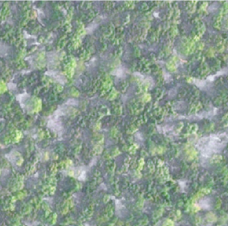
\includegraphics[width=0.75\linewidth]{Picture1.png}
  \caption{Satellite Image For Testing}
  \label{fig:my_label}
\end{figure}

 Figure 2 below is Figure 1's corresponding visualization with the model's predicted dead tree locations. In Figure 2, magenta circles represent ground truth centroids of dead trees, the green plus sign indicates true positives of dead tree centroids accurately predicted by the model, and the yellow line indicates distances between ground truth dead trees and correctly predicted dead trees by the model. The yellow triangle in Figure 2 indicates a false positive, where the model predicted a dead tree where there wasn't one, and the magenta circle with a black border indicates a false negative, in which case an actual dead tree centroid existed, but the model did not predict it.

\begin{figure}[htbp]
  \centering
  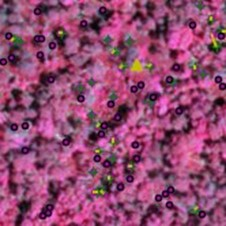
\includegraphics[width=0.75\linewidth]{Picture2.jpg}
  \caption{False Color Visualizations w/ Predicted Annotations}
  \label{fig:my_label}
\end{figure}


\section{Methodology}

Our team adapted the neural network used by Ventura et al. that detects trees in urban environments to detect dead trees in satellite images. The model by Ventura et al. describes the architecture of the neural network that we adapted. The  architecture diagram is described in Figure 3. 

\begin{figure}[htbp]
  \centering
  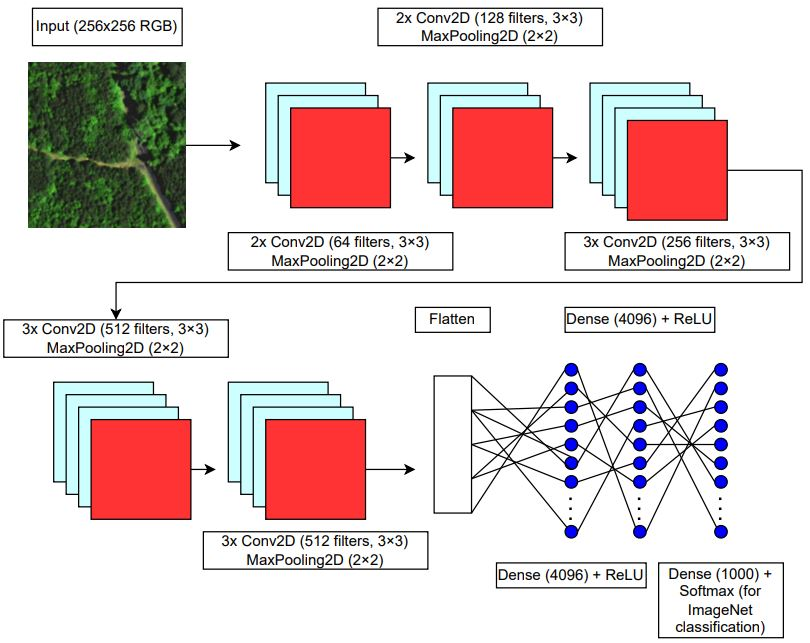
\includegraphics[width=\linewidth]{VGG_diagram.JPG}
  \caption{VGG Architecture Diagram}
  \label{fig:my_label}
\end{figure}

Our initial results from directly implementing the model are as follows. 

\begin{table}[htbp]
  \centering
  \begin{tabular}{lcc}
    \hline
    \textbf{Metric} & \textbf{Testing} \\
    \hline
    Precision & 0.762 \\
    Recall    & 0.589 \\
    F-Score   & 0.663 \\
    RMSE [px] & 2.70 \\
    \hline
  \end{tabular}
  \caption{Baseline VGG16 Performance}
  \label{tab:metrics}
\end{table}

A batch of data for our model consists of a 256 x 256 satellite image with red, blue, green, and alpha channels, and an annotation image with non-black pixels representing vertices of polygons circumscribing dead trees. Our model uses 2D convolutional layers to detect features of dead trees. The model also uses pooling layers to look at specific areas of an image at a time and combine portions of the image to reduce the dimensions, ensuring a focus on the most important features. Finally, the model adds an attention map to focus on regions where dead trees are likely to be located and a confidence map to show the likelihood of dead trees at any given pixel. 

In this architecture, the loss function is broken down into two parts, Mean Squared Error (MSE) loss and Binary Cross Entropy (BCE) loss. MSE is the main loss function and compares predicted and actual ground truth confidence maps. The ground truth map includes indicators that pixels represent centroids of dead trees. The ground truth map is compared to the model’s predicted map of probabilities whose pixels represent centroids of dead trees. MSE loss is used to see how much the model differs from the ground truth when searching for dead trees in the training and validation images. The BCE loss focuses on the attention map, determining how well the predicted regions of dead trees match actual regions that have dead trees. Our final loss calculation adds the MSE loss to a weighted BCE loss (depending on how important we find each loss) to obtain our total loss function as seen in Figure 2. 

We use the architecture of Ventura et al. and have applied our deep learning knowledge to improve this architecture and the prediction of centroids of dead trees by our neural network. We evaluated the performance of our model and improved our model and its predictions by examining the loss curves derived during training and validation. We also focused on improving precision, recall, F1 score, and the root mean square error (RMSE) calculated during validation and testing. We also doubled the weight of attention loss and updated activation to additionally improve the model. Below in Table 2 are some of our best testing performance metrics without data augmentation:


\begin{table}[htbp]
  \centering
  \begin{tabular}{lcc}
    \hline
    \textbf{Metric} & \textbf{Testing} \\
    \hline
    Precision & 0.803 \\
    Recall    & 0.784 \\
    F-Score   & 0.793 \\
    RMSE [px] & 2.763 \\
    \hline
  \end{tabular}
  \caption{Best testing metrics without augmentation}
  \label{tab:metrics}
\end{table}


Our primary performance metrics for the model are precision, recall, F1 score, and RMSE. Precision measures the number of true positives divided by the number of total positives in the model, both true and false. In the scope of our project, precision represents how many of the predicted dead trees are actually dead trees. Our baseline precision of about 0.80 indicates that about 80\% of the predicted dead trees in the model were indeed dead trees according to ground truth. Recall indicates our model’s ability to capture as many dead trees as possible, for which we were able to capture 78\% using our baseline model. Our F1 score of 79\% represents the performance of the model when combining precision and recall. Finally, we are using RMSE to compare the distances between true positive predictions of dead trees and the ground truth map counterparts. We had a goal of achieving 80\% F1 score on the testing data, with balanced precision and recall. While this baseline model performed well, we had to make further improvements to achieve these goals. 

\section{Alternative Architectures} 

\subsection{ResNet50}

To try improving our results, we swapped out Ventura’s VGG backbone with ResNet50, a deeper neural network that theoretically can better map complex relationships. The model also alleviates the vanishing gradients problem with its novel skip connection idea, making it one of the premier deep CNNs. The architecture diagram for the ResNet model is shown in Figure 4 to the right.

\begin{figure}[htbp]
  \centering
  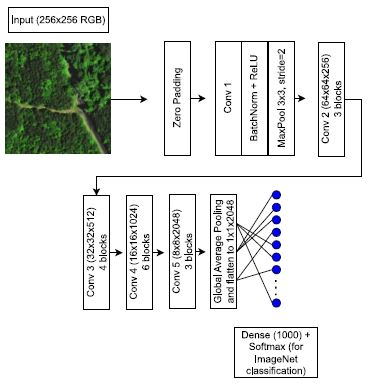
\includegraphics[width=0.9\linewidth]{ResNet.JPG}
  \caption{ResNet Architecture Diagram}
  \label{fig:my_label}
\end{figure}
\FloatBarrier

While ResNet50 converged faster than VGG in training, its test performance results are worse: 


\begin{table}[htbp]
  \centering
  \begin{tabular}{lc}
    \hline
    \textbf{Metric} & \textbf{Testing} \\
    \hline
    Precision & 0.810 \\
    Recall    & 0.654 \\
    F-Score   & 0.723 \\
    RMSE [px] & 2.83 \\
    \hline
  \end{tabular}
  \caption{Testing metrics ResNet.}
  \label{tab:testing_metrics}
\end{table}



\subsection{EfficientNet}

We also experimented with EfficientNet, another widely-used deep CNN that uniformly scales dimensions like width, depth, and resolution. Figure 5 below is the architecture diagram for EfficientNet:

\begin{figure}[htbp]
  \centering
  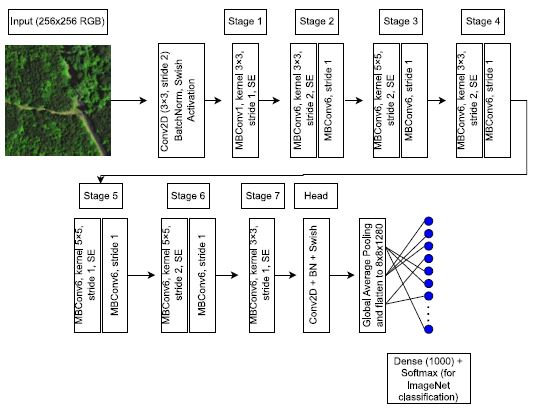
\includegraphics[width=\linewidth]{EfficientNet.JPG}
  \caption{EfficientNet Architecture Diagram}
  \label{fig:my_label}
\end{figure}

The best results from this model are as follows:

\begin{table}[htbp]
  \centering
  \begin{tabular}{lc}
    \hline
    \textbf{Metric} & \textbf{Testing} \\
    \hline
    Precision & 0.764 \\
    Recall    & 0.714 \\
    F-Score   & 0.738 \\
    RMSE [px] & 2.97 \\
    \hline
  \end{tabular}
  \caption{Testing metrics EfficientNet.}
  \label{tab:testing_metrics}
\end{table}

The alternative architectures performed worse overall than the VGG model despite the deeper architectures and keeping attention and confidence map outputs. This suggests that although deeper, these alternative architectures may not have captured the domain-specific features as effectively as the customized VGG. A future step would be to customize these alternative architectures to see if we get improved results.

\section{Data Augmentation} 

As described in previous sections, we looked to implement data augmentation as a method for increasing the performance of our model. We believed this would increase the robustness of our model to potential changes in the seasonality of satellite images and reduce overfitting to our training set that is limited to East Coast satellite images. In the implementation of data augmentation, we were able to expand the scale of the dataset by performing several transformations to the images. Specifically we applied 90-degree rotations, vertical flips, brightness and contrast changes, and image cropping. This allowed us to expand the data set by a factor of 4, which allowed for more robust training. We also randomized the application of these data augmentations to allow for further variation in the data. This will build resistance and robustness into the model when our sponsors expand their research outside of the East Coast of the United States. Overall, data augmentation resulted in slight improvement in testing performance metrics, such as an F1 score of 0.795.

 
\section{Loss Functions}

In this section, we describe the loss functions used for training and evaluating our model. The baseline losses are Mean Squared Error (MSE) and Binary Cross Entropy (BCE). MSE is used for regression tasks where the target outputs are continuous values, such as the predicted confidence map for tree centers. BCE is used for binary classification tasks, for instance identifying regions of tree pixels versus background.

Although these baseline losses are effective in general settings, challenges such as severe class imbalance, small object detection, and segmentation noise motivated the exploration of alternative loss functions. In the following subsections, we describe each loss, provide the governing equations, and present the experimental results obtained on both the full and reduced datasets.

\subsection{Binary Cross Entropy}

Binary Cross Entropy (BCE) is a standard loss function for binary classification tasks. It measures the dissimilarity between predicted probabilities and ground-truth binary labels. The BCE loss is defined as:

\[
\mathcal{L}_{\text{BCE}}(y, \hat{y}) = -\left( y \log(\hat{y}) + (1 - y) \log(1 - \hat{y}) \right),
\]
where \( y \in \{0, 1\} \) denotes the true label and \( \hat{y} \in [0, 1] \) the predicted probability.


\subsection{Binary Focal Cross Entropy}

Binary Focal Cross Entropy modifies the BCE loss by down-weighting the loss assigned to well-classified examples, focusing training on harder examples. The focal loss formulation for binary classification is:

\[
\mathcal{L}_{\text{Focal}}(y, \hat{y}) = -\alpha (1 - p_t)^\gamma \log(p_t),
\]
where:
\[
p_t = 
\begin{cases}
\hat{y}, & \text{if } y = 1, \\
1 - \hat{y}, & \text{if } y = 0,
\end{cases}
\]
\(\gamma\) is the focusing parameter controlling the down-weighting (commonly set to 2), and \(\alpha\) is a balancing factor between classes.


\subsection{Categorical Focal Cross Entropy}

Categorical Focal Cross Entropy generalizes the focal loss to multi-class classification tasks. It is defined as:

\[
\mathcal{L}_{\text{Focal, Categorical}} = -\sum_{c=1}^{C} \alpha_c (1 - \hat{p}_c)^\gamma y_c \log(\hat{p}_c),
\]
where \(C\) is the number of classes, \(y_c\) is the ground-truth label for class \(c\) (using one-hot encoding), \(\hat{p}_c\) is the predicted probability for class \(c\), and \(\alpha_c\) is the balancing weight for class \(c\).


\subsection{Dice Loss}

Dice Loss is tailored for segmentation tasks, particularly when dealing with highly imbalanced classes. It directly maximizes the overlap between the predicted segmentation and the ground-truth mask. The Dice Loss is given by:

\[
\mathcal{L}_{\text{Dice}}(y, \hat{y}) = 1 - \frac{2 \sum y \hat{y} + \epsilon}{\sum y + \sum \hat{y} + \epsilon},
\]
where \(\epsilon\) is a small constant to avoid division by zero.




\subsection*{Summary}

Experimental results from testing demonstrate the performance of the various loss functions. On the data set, BCE achieved a balance between precision and recall, with the best performance in the data set.

Binary Focal Cross Entropy (BFCE) showed similar recall metrics to BCE on the dataset, where it enhanced the detection of smaller structures without sacrificing precision.

Categorical Focal Cross Entropy (CFCE) performed poorly in most metrics with the exception of recall which was higher than the other loss functions. However, it requires more careful hyperparameter tuning. The added complexity also introduces slower training convergence.

Dice Loss performed the most consistently across varying datasets with and without augmentation. Performance wise the dice loss function performed closest to the baseline BCE model. 

In conclusion, BCE showed the most promising results in terms of both segmentation quality and stability, while the other loss functions exhibited strengths in certain areas but with trade-offs in terms of training dynamics and performance. 

 
\section{Results}

We were successfully able to adapt and improve the performance of our model to our objective, the detection of dead trees on satellite imagery. As discussed in the methodology section, we applied several improvements to the base VGG model, and these improvements allowed for us to achieve the following results:

\begin{table}[h]
\centering
\caption{Summary of Best Results}
\label{tab:dice_full}
\begin{tabular}{lcccc}
\toprule
Metric & Precision & Recall & F1 Score & RMSE (px) \\
\midrule
Value  & 0.775 & 0.816 & 0.795 & 2.82 \\
\bottomrule
\end{tabular}
\end{table}


Our sponsors had the goal of achieving around an 80\% F1 score on the test set and having a balanced result with recall and precision. We were able to successfully achieve these goals, getting a best F1 score of 79.5\%, and having similar results across precision and recall, meaning that our model successfully predicted most dead trees in the data, and predicted them without too many false positives. In Figure 6, to the right, is a visualization of this high precision where the rate of actual dead trees per hectare is highly correlated with the rate of predicted dead trees per hectare:

\begin{figure}[htbp]
  \centering
  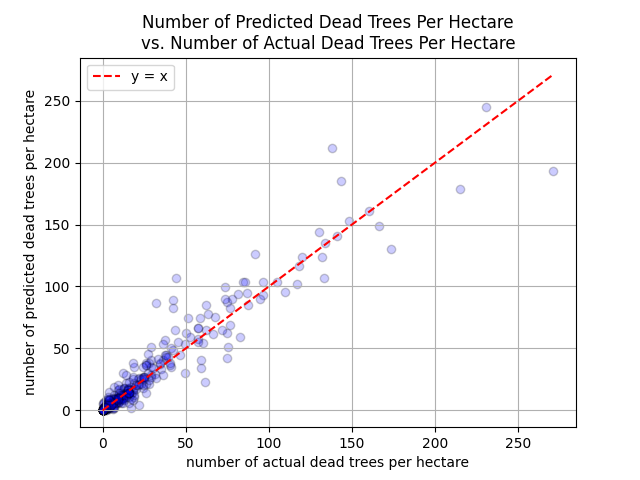
\includegraphics[width=\linewidth]{scatter_plot.png}
  \caption{Visualization of Final Model High Precision}
  \label{fig:my_label}
\end{figure}
\FloatBarrier




\section{Discussion}
Our project demonstrates the feasibility of adapting an urban tree detection model for the novel task of detecting ghost forests from satellite imagery. By retraining and modifying the Ventura et al. architecture, we achieved promising results, with our VGG-based model reaching an F1 score of 0.795 and precision of 0.775 with a recall of 0.816 on the testing dataset. These metrics indicate that a substantial majority of detected trees correspond to true dead trees, which is critical for generating reliable ghost forest maps. 


Despite these successes, challenges remain. Our attempt to use a deeper ResNet50 backbone did not yield better performance, underscoring the importance of model choice relative to the dataset. Moreover, improving spatial precision and generalizing to diverse conditions will be critical in moving from individual dead tree detection to comprehensive ghost forest mapping past the East Coast of the United States.
Primary future work will include combining the alternative architecture methods and loss functions with the data augmentation we added.
Post-processing methods to aggregate dead trees into ghost forest regions and time series analysis to track forest decline will also be important next steps. We additionally plan to make the EfficientNet and ResNet architectures more customized to our data since we noticed their poorer probability maps and worse results than the VGG16 model.
Finally, we will conduct deeper hyperparameter searches, including trying different learning rates, optimizers, and loss function compositions, which could further improve model performance. 

\section{Conclusion}
In this project, we successfully adapted and improved upon existing deep learning methods to detect ghost forests along the East Coast of the United States. Our approach, based on adapting the VGG architecture, achieved strong testing performance. We demonstrated that models trained on small-sized annotated satellite imagery datasets can generalize to unseen data through careful model design, rigorous data processing, and effective data augmentation.

By building an accurate and scalable pipeline for ghost forest detection, we contribute valuable tools that researchers and policymakers can use to better understand and combat coastal forest loss, supporting efforts to protect vulnerable ecosystems and communities across the United States.
\bibliographystyle{IEEEtran}
\bibliography{references}

\end{document}
